\documentclass[a4paper]{sbgames}               % final
%\usepackage[scaled=.92]{helvet}
\usepackage{times}
\usepackage{graphicx}

%% use this for zero \parindent and non-zero \parskip, intelligently.
\usepackage{parskip}

%% the 'caption' package provides a nicer-looking replacement
\usepackage[labelfont=bf,textfont=it]{caption}

\usepackage{url}
\usepackage[]{algorithm2e}
\usepackage{array}
\newcolumntype{L}{>{\centering\arraybackslash}m{3cm}}

%% Paper title.
\title{Developing an Accessible One-Switch Game for Motor Impaired Players}


%% Author and Affiliation (multiple authors). Use: and between authors

\author{Fernando L. Souza: Lucas C. Medeiros: Marcos F. Parreiras}

%\affiliation{Departamento de Computa\c{c}\~{a}o \\
%        Centro Federal de Educa\c{c}\~{a}o Tecnol\'{o}gica de Minas Gerais \\
%        Belo Horizonte, Brasil
%}

\affiliation{ Centro Federal de Educa\c{c}\~{a}o Tecnol\'{o}gica de Minas Gerais, Departamento de Computa\c{c}\~{a}o, Brasil
}

\contactinfo{nandolcs@hotmail.com \\
             *cmedeiros.lucas@gmail.com \\
             *marcosfparreiras@gmail.com
}
%\contactinfo{author1@email.com \\
%             author2@email.com
%}
%% Keywords that describe your work.
\keywords{accessibility. motor impairments. digital game. one switch.}

%% Start of the paper
% Attention: As you need to insert EPS images in Postscript, 
% you need to insert PDF images into PDFs. 
% In the text, extensions cancbe omitted (latex use .eps, pdflatex get .pdf) 
% To convert them: epstopdf myimage.eps
\begin{document}

%\teaser{
 % 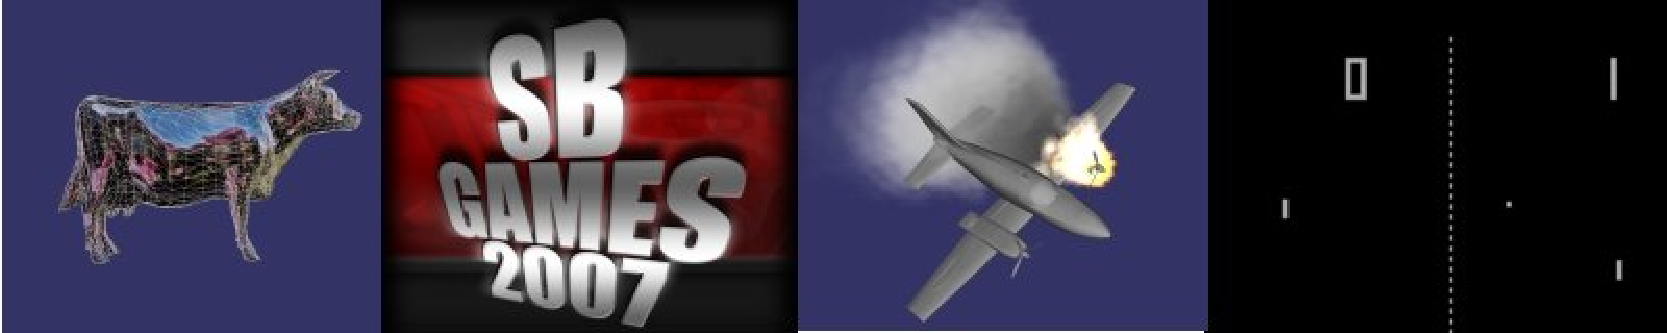
\includegraphics[width=\linewidth]{sample.pdf}
  %\caption{Optional image}
%}

%% The ``\maketitle'' command must be the first command after the
%% ``\begin{document}'' command. It prepares and prints the title block.

\maketitle

%% Abstract section.

\begin{abstract}

Digital games typically require a fair amount of sensory and motor skills.  However, not every player can receive stimuli and provide feedback at the usually necessary extent and rate.  About 24\% of the Brazilian population has some degree of a disability, of which 7\% has motor impairment.  This work describes the creation of a simple digital game that is accessible for people with motor impairments through the use of the one-switch technique, which is the use of a single key or button to provide all input to the game. Our goals included putting the accessible and the traditional game modes in equal footing in terms of freedom and difficulty and evaluating the effort to develop the one-switch version.  Usability tests were carried out to users who have some motor disability and to users who do not. Results showed that the use of a single key does enable people with varying motor difficulty to play a game with more balanced competitiveness compared to people who are not disabled and also that the gaming experience was satisfactory for both user groups.
\end{abstract}

%% The ``\keywordlist'' command prints out the keywords.
\keywordlist
\contactlist

\section{Introduction}

% Contextualize
More than ever, people have been playing digital games. A survey conducted by the Entertainment Software Association \shortcite{ESA2015} showed that 51\% of the households in the United States own a dedicated gaming console and that 42\% of the population play video games regularly. In addition to that, gamers have been spending more time playing games. Nielsen \shortcite{Nielsen2014} showed that there was an increase in weekly play time of 10\% from 2011 to 2012 and of 12\% from 2012 to 2013. There is also a plethora of games available to play in many different platforms, ranging from more casual genres to more time consuming ones. Most of them require a lot of motor and sensory skills due to their specific purposes, complex gameplay and need of attention \cite{bierre2004accessibility}.

New programming tools emerge everyday and they make it possible to improve digital game quality. Through the Internet, people from all over the world can have access to lots of games providing fun, learning, and improvement in their quality of life. Many of them are also being used in treatments of diseases and sequelae with very interesting results \cite{kato2010video,baranowski2008playing}.

% Motivate
However, people with some form of disability might have difficulties playing games which are not accessible. Non accessible game is one that imposes barriers to players because of different health conditions they might permanently have or might be going through \cite{yuan2011game,Coutinho2011a}. Being able to choose to play a game should be an option granted to everyone, specially in societies that strive to become inclusive \cite{bierre2004accessibility}.

A survey conducted by WHO \shortcite{world2012relatorio} indicates that more than one billion people (almost 15\% of the world population) has some kind of disability. In Brazil, that percentage is even higher, of 24\% \cite{demografico2010caracteristicas}. That is a considerable amount of people and it motivates the development of accessible games to reach that portion of the population, if not for the reason of inclusion, at least as a measure of expanding the target audience and a chance to increase profit in the game industry.

Some studies have been done in order to provide accessible games to people, usually targeting one type of disability: visual, auditory, mobility or cognitive \cite{Coutinho2012,Coutinho2011a,Gerling:2013:KWW:2468356.2479609,Gerling:2012:FMG:2207676.2208324}. A white paper from the Game Accessibility Special Interest Group of the International Game Developers Association \shortcite{IGDA2004} describes how gaming experience is affected by different types of disabilities and presents some accessibility guidelines. Of a total of 19, 16 instructions tackle visual impairments and only 4 aim at motor or hearing disabilities.

In Brazil, about 7\% of the population is affected by some degree of motor impairment \cite{demografico2010caracteristicas}. Depending on the extent of the limitation of movements, a player might be able to hit just a single key or button to interact with games. In that case, the suggested guideline is to use the one-switch technique \cite{IGDA2004} to allow the interaction with all game screens using a single button. The website OneSwitch.org.uk \shortcite{oneswitch} is devoted to disclosing information on one-switch games.

To be one-switch accessible, games need to automate some of its aspects, such as the character movement, shooting time, aiming etc. To simplify the controls, some games reduce the extension of interaction by plainly removing some of the options a player would have in case the game was not being played in the one-switch mode. For example, an one-switch accessible remake of the game Frogger \shortcite{frogger}, listed by OneSwitch.org.uk site, only lets the main character go up or downwards, not allowing movements to the right and left \cite{froggeracessivel}. Besides reducing the player flexibility and freedom of controlling the main character, removing control options might also derange the game difficulty balance by making it easier or harder than the non-accessible mode, if one exists.

% Present goals
Focusing on accessibility for motor impaired players, this work aimed at developing a simple game from the ground up to evaluate the feasibility and pertinence of the one-switch technique. In particular, we were interested in building a game in which both the traditional and the accessible input modes would be in equal footing, as much as possible, in terms of freedom of controls and difficulty level.

% Bit of conclusion
To achieve that goal, a simple game was developed, featuring both an accessible one-switch mode and a traditional one. Having users with and without motor disabilities to assess the game, it was found that the one-switch technique was efficient to promote good accessibility for people with some motor difficulty and also that both game modes were balanced in difficulty and of player preference. 

% List contributions
Contributions of this work include the public release of the free and open-source\footnote{The source code of the game is hosted publicly at the URL: \nolinkurl{http://github.com/luccascm/zac-esquilo/} and can be further developed and distributed by anyone} game, which can be played through a web browser\footnote{The game can be played in most recent browsers through the URL: \nolinkurl{http://luccascm.github.io/zac-esquilo/}}, and also, as a result of the adopted methodology, a proof of concept that one-switch versions of games can and should strive to be as flexible as the traditional game modes.

\section{Related Work}
\label{sec:related-work}
% how motor impairment impacts the gaming experience (2.1 (interaction model) + 2.1.4) \cite{IGDA2004}
There are many kinds of impairments that can limit a person trying to play a game. The most common types are visual, hearing, motor or cognitive issues. A game interaction model presented by Yuan et al. \shortcite{yuan2011game}, proposed through the  analysis of different game genres, describes how a player interacts with a game. The model is illustrated by Figure \ref{fig:gameInteractionModel} and described next.

\begin{figure}['h']
	\centering
	\caption{Game interaction model per Yuan et al. \shortcite[adapted]{yuan2011game} }
	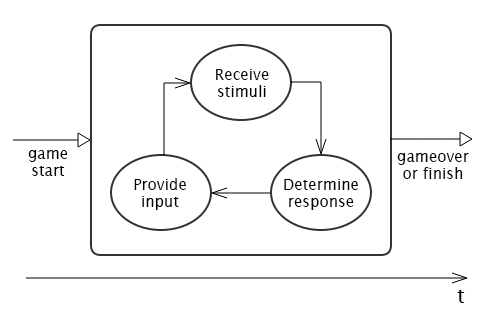
\includegraphics[width=0.32\textwidth]{./images/game-interaction-model.jpg}
  	\label{fig:gameInteractionModel}
\end{figure}

\begin{description}
\item[Receive stimuli] Visual, auditory and haptic are the three forms a game can provide stimuli. Being able to play the game depends on being able to receive primary stimuli. Secondary ones are provided as an extra since the player can still play the game but gaming experience may be reduced if they are not provided or received.   
\item[Determine response] The player must think and cognitively determine which in-game response(s) to provide according to the set of stimuli provided by the game. These actions are specific to each game genre.
\item[Provide input] Having decided the response, the player must physically provide the input through the input device used to interact with the game. Most games uses physical device such as keyboard, mouse or controller.
\end{description}

New stimuli may be provided after these three steps having been performed successfully. The steps are repeated until the game finishes or the player win, lose or quit it. \cite{yuan2011game}

Paralysis, neurological disorders, repetitive stress injury, age related issues, lack of mobility and lack of steadiness are examples of motor disabilities. Players with this kind of impairment may have difficulty to provide input physically. In these cases, a game that requires a lot of mouse motion, very quick responses or complex control with different buttons is not suitable to them \cite{IGDA2004,Coutinho2011a}.

% one switch technique (2.2, but very condensed)
Using a single switch to control the actions of the game such as choosing options and moving the main character might help or even enable motor impaired players to play games. Colven and Judge (p.8) \shortcite{colven2006switch} allege that \textit{``Switch systems must, therefore remain flexible in terms of types of control, scanning and response so that they can always match the user's needs.''} and they show a few ways to present choices and to make selections. The \textbf{scanning} method involves moving the focus from one item/group to the next in a set of order. In simple scanning, items are highlighted one at a time. It is very important to make it clear to the player which option is focused so they can make the choice they really want to do. In digital games context, choices are usually made by the keyboard or mouse and sometimes with extra hardware. With scanning, the options are focused for some period of time allowing the player to press a key or button to make the selection. The focus usually moves from top left to down right corner.

This technique does not always work for every screen in a game, specially for action-based ones, as the player typically needs to make split second decisions and might not have spare time to wait for the focus to get to the desired option. Alternatively, different solutions have been proposed \cite{beukelman2005augmentative}. One of them is to make an automation of control so that the single key has different effects on the character according to the situation of the game. The PORTEM game \footnote{\nolinkurl{http://www.mirrowgames.com/en/portem.php}}, for example, is a 3D game in which players explore a city and do small tasks. The direction of the movement is defined by pressing and releasing the key and the selection changes along the options forward, left and right.

% related works proper (Jönsson 2005; Folmer et al. 2011)
Folmer et al. \shortcite{folmer2011navigating} expose a scanning system called hold-and-release to control the navigation of an avatar in the 3D virtual world of the game Second Life\footnote{\nolinkurl{http://www.secondlife.com}}. The focus of the work was at navigating the player's avatar since this game does not need quick responses like action or FPS\footnote{First Person Shooter} games do. The technique used consists in keeping the activated input highlighted until it is released (using another switch activation) and mixing inputs to input already activated, so the player can move FORWARD + LEFT or BACKWARD + RIGHT for example. This multistep selection is potentially more efficient as players can adjust the movement of an avatar without having to stop it when selecting a mixed input option.

A different strategy can be found on J{\"o}nsson \shortcite{jonsson2005if}, that presents an evaluation of the use of eye tracking use in computer games, technique in which eye movements and winking are monitored by a camera and used to determine input. It was tested in three prototypes, all FPS games. The eyes were used to aim, to shoot and to control the camera. The result of the usability study showed that interaction with the eye was easy to learn, very fast and natural. The conclusion suggests that eye-based interaction may be successful in computer games but it needs to be further developed.

In the context of this work, a simple game was developed  using one-switch technique based on the game Frogger \shortcite{frogger} with a different theme, as the player has to guide a squirrel back to the forest instead of a frog. A scanning system is used to present choices in which each option is highlighted by changing the button background color and a squirrel icon points the focused option. When the focus is moved it is played a short sound as a secondary stimuli. It was decided to automate character movement with an algorithm which makes it possible to the player moves up, down, left or right which differs from accessible version of Frogger mentioned previously that only lets the main character go up or downwards. The presentation and use of scanning and automation of control techniques are good scientific contributions provided by this work as it demonstrates that those methods are, in fact, useful to reach a good level of accessibility regarding motor impairments.

\section{Methodology}
\label{sec:methodology}

The final goal intended from the methodology consisted of evaluating the use of the one-switch input method for action-based games and the assessment of the balancing between game modes.

The game developed has three different modes. The first one, traditional and non accessible in which players use the mouse to select options and directional arrows keys to control the main character. The others are accessible modes in which the space bar key is used to make selections and to move the character. The difference between them is that in one the movement algorithm allows the squirrel to move to one of the four directions, up, down, left or right and in the other one it is only possible to go up. Those modes are related to the objectives proposed so it becomes possible to compare the gameplay in accessible and non accessible modes to evaluate the pertinence of the one-switch technique and to check if both input modes are in equal footing in terms of freedom of controls and difficulty level. Having two accessible modes are important to assess the effects that the movement algorithm brings to game allowing the main character to move in different direction or only up.

In addition, the game provides the possibility of defining the time in which the focus is switched among options in scanning and turning on and off the game sounds. There is also a instruction screen which explains how to play the game.

For the evaluation, a user test was conducted with six people, three of which have some level of motor impairment and the others do not. In the test, the users were conducted to follow a script with seven tasks to be executed, which encompassed playing the game in the three game modes and also interacting with the accessory screens (main menu, options etc.). Those were listed in order to test the accessibility all over the game and the gameplay.

Before the test, a questionnaire was filled out to determine the profile of the users, with questions about their previous gaming experience and what type of health conditions they might have. After the test, another questionnaire and a quick informal interview were carried out to the users. There were questions comparing the fun and the challenge level of the three game modes proposed and asking if the players had enjoyed the game and if they would play it again.

\section{Development}
\label{sec:development}
The first step of this project was to specify some aspects and requirements to develop a game in which the use of one-switch could be well evaluated. It was decided to create the game using HTML5 \footnote{HTML5 is the newest and most recent version of HTML} and JavaScript. HTML was used so the game can be played in most recent browsers in devices with different operational systems and architectures. JavaScript provides the game some interesting features such as animations and its oriented object features helps in structuring the game source code.

At first, the game was developed with traditional input mode only having the one-switch version been based in a module that was reused in all the game screens either to present choices or to move the character.

\subsection{OneSwitchManager Class}
\label{sec:OneSwitchManagerClass}
This class has essential functions to make the game accessible to motor impaired players. It controls the focus transition throughout the options according to the time defined in the game options by doing the automatic switching among them. In each screen a oneswitchmanager object is created with the following: an array with objects that represents the options of that screen, the switching time interval and a boolean that defines if sound effects are on or off. The class has methods start and stop the switching, to change the state of each option between selected or not and to call the action of the option activated when the single key is pressed.

For the game screen proper, it was decided to automate the player movement as the game is action-based and the algorithm of decision is described next.

\subsection{Player Movement Algorithm}
\label{sec:MovementAlgorithm}
An algorithm was proposed to improve player movement along the scenario. It determines the direction of movement when the switch is pressed. With this algorithm the player can move in one of the four basic directions (up, down, left, right) depending on the game state at the time of activation.

\begin{algorithm}[ht]
\caption{Algorithm to determine character movement direction}
 \KwData{game state}
 \KwResult{movement direction}
 initialization\;
 \eIf{can move up}{
   go up\;
   }{
   \eIf{can move side}{
    go left or right randomly\;
   }{
    go down\;
   }
  }
\end{algorithm}

\subsection{The Game \textit{``Zac - O Esquilo''} (The Squirrel)}
The game goal and theme consist on directing a squirrel called Zac back home in the forest, by crossing a busy road and navigating a river. The game starts with three lives. The player guides the main character, which starts at the bottom of the screen and should reach the forest at the top. Zac dies if hit by a vehicle or if he moves into the water. Some logs float on the water and they must be used by Zac to cross the river.

Upon starting the game, a splash (branding) screen is shown for a few seconds, after which a game mode selection screen is presented to the player. The accessible, one-switch mode is activated by default. This mode uses scanning to present choices to user. The options are highlighted and a small squirrel icon points to the focused one. The default time to switch options is two seconds. On the options screen, the player can change the wait time of the scanning to 1, 2 or 3 seconds, as well as change to another game mode. In the game scene, pressing the single key will move the main character to the direction returned by the movement algorithm. Figure \ref{fig:ZacGameScenes} illustrates some of the game screens.

\begin{figure}['htc']
	\centering
	\caption{``Zac - O Esquilo'' game screens (in Portuguese)}
	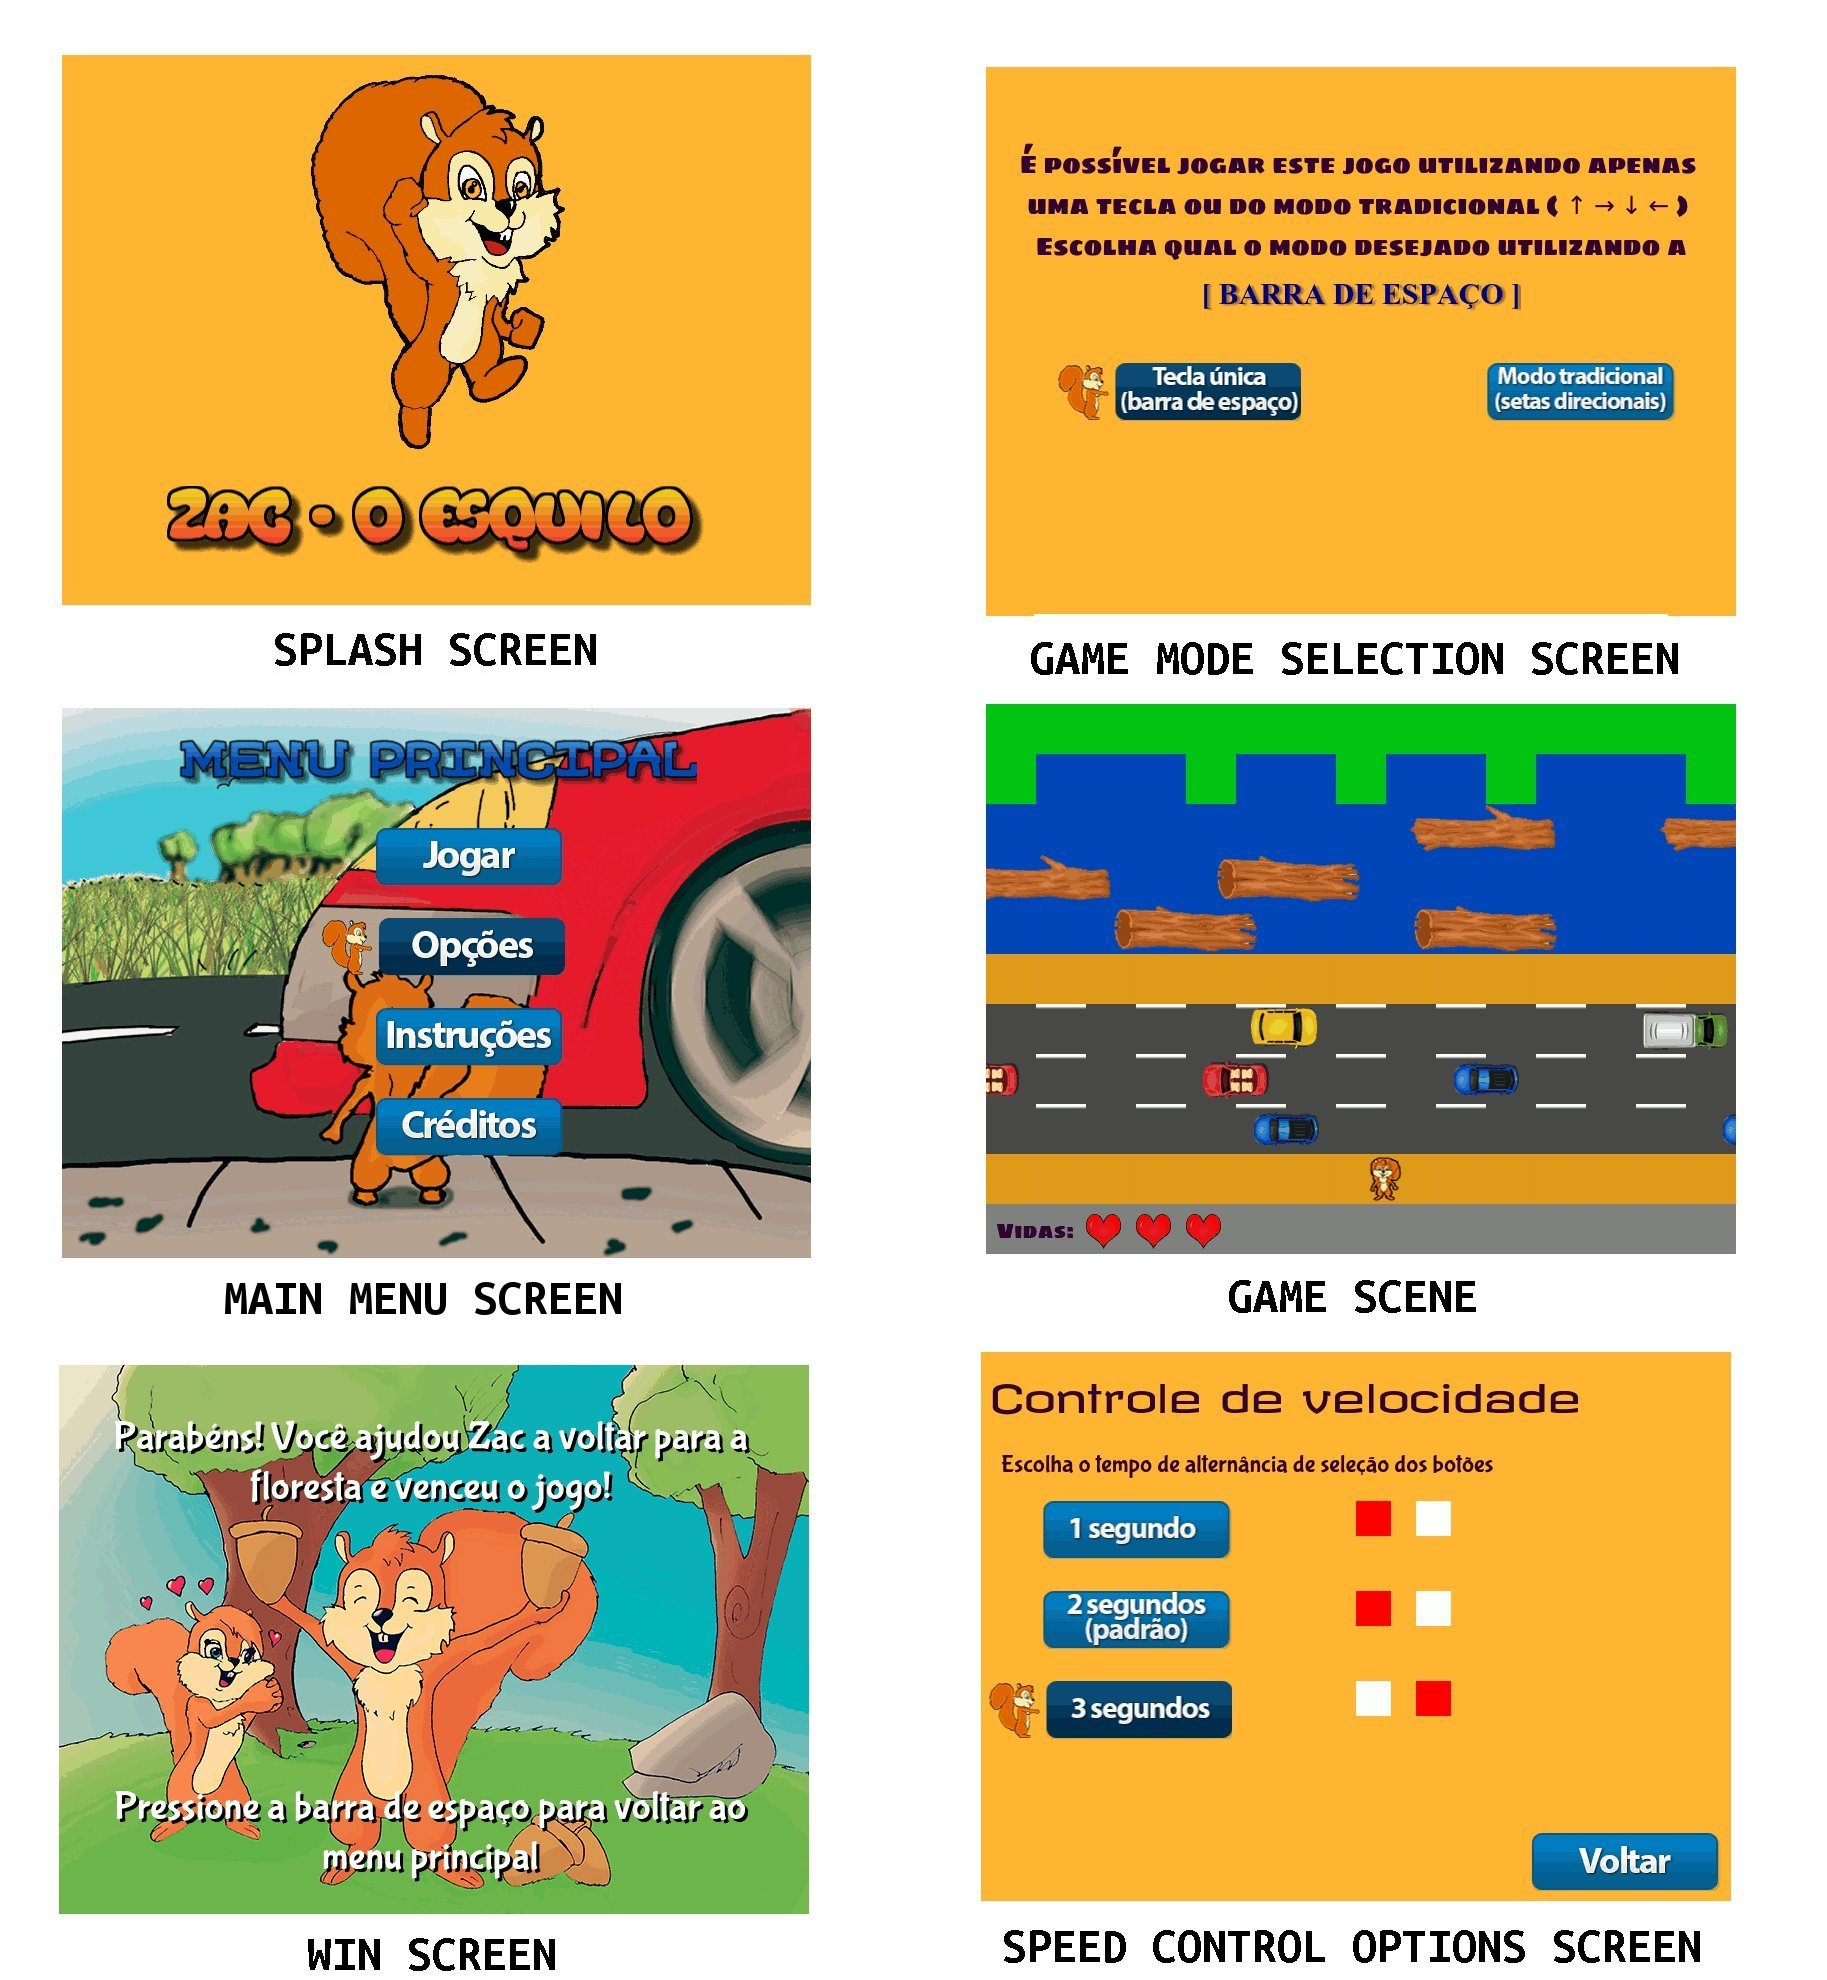
\includegraphics[width=0.35\textwidth]{./images/zac-scenes.jpg}
  	\label{fig:ZacGameScenes}
\end{figure}

\section{Evaluation}
\label{sec:evaluation}
Based on Nielsen' \shortcite{nielsen2000you} guidelines, a usability evaluation was conducted with six people. First, a pre-test questionnaire about their profiles was applied. For the test proper, they were presented a script with the seven tasks listed next.

% list of tasks
\begin{enumerate}\label{tasksList}
  \item You decide do play the game in one-switch mode. So, enter the game in this mode, read the instructions and return to main menu.
  
  \item You realize that game music can take your attention off but you want to keep sound effects on. So, turn off game music and go back to main menu.
  
  \item Now that you have already read the instructions and turned the music off, you want to play the game. Therefore, complete the game in one-switch mode.
  
  \item You know that there is another game mode, traditional, using directional arrows and mouse and decide to play the game in this mode. Change game mode to "traditional" and go back to main menu.

  \item Now that you have changed mode, you want to test it. Complete the game in traditional mode.
  
  \item After completing the game you have the curiosity to see who were the developers of the game. Thus, read the game credits and return to main menu.

  \item The change made in game proposed a new one-switch game mode. Now, complete the game in alternative one-switch mode.

\end{enumerate}
After the test, another questionnaire and an informal interview were conducted to assess the fun and challenge level of each game mode and if the users have liked the game and would play it again. Each test was done separately, in a partially controlled environment, preventing other users to see any part of the experiment.

The participants were men and women between 17 and 92 years old. Three users (D1, D2 and D3) have some level of motor impairment and the others (P1, P2 and P3) do not. D1 is slightly developmentally disabled and has a fracture in one of his hands. He had already played an accessible FPS game using the one-switch technique. D2 has developed cerebellar ataxia during adolescence and started to lose movements and to suffer from tremor of hands at the age of 25. D3 has incomplete quadriplegia and cerebral palsy. Despite the varying degrees of motor impairments, D1, D2 and D3 desired and did play the game including in the traditional mode.

Regarding gaming experience, all users had already played any digital game, except for P1. P2 was the most experienced player and P3 is the oldest one and has only played chess and checkers. D1 has good experience with video-game and great knowledge about shooting and fighting games. D2 and D3 had little contact with digital games.

All users played the three modes of the game. P2 is the only one, among all participants, who did not die when playing the game in one-switch mode. D2 was the only one who did not finish the game in this mode. The post-test questionnaire questions about which game mode was more fun and which one was more challenging had a good variety of responses and no mode was much more preferred than any other. All players also answered that they would play the game again except for D1 who said that he did not like the game genre. Those facts show that the one-switch technique revealed itself efficient to this game. In addition, the results indicate the game has good usability and quite well equal footing between game modes.

\section{Conclusion}
\label{sec:conclusion}
% Recap and conclude
Non accessible games demand efforts and skills that impose barriers to a person with some level of disability. This project proposed an evaluation of one-switch technique to motor impaired players in an accessible game developed in the context of this work. One-switch games are the ones which only a single switch is used to control all actions in the game.

Developing a game with this technique requires several modifications on presenting choices and character navigation. But it brings lots of benefits such as promoting more socialization and inclusion of people with motor impairments, giving them the opportunity to choose either to play the game or not.

Through the game developed it was possible to assess the feasibility and pertinence of the one-switch technique. The game was first developed in its non accessible version and then it was included strategies to make the one-switch game input mode work properly. A user test was conducted to evaluate whether the use of this technique actually makes the game accessible to players with some motor difficulty. From the results of the test, carried out with six users, three of which were motor impaired players, along with the post-test questionnaire answers it could be concluded that one-switch technique showed itself very useful in order to make the game accessible to motor impaired players. Furthermore, it was shown that this technique makes the feasibility of having traditional and accessible mode in equal footing in terms of game control and difficult level more easily achievable.

Having the game developed with traditional input mode first, the main difficulty in doing the one-switch version was to create the scanning mechanism and the algorithm to automate the direction of movement as the game logic was already set. Once created it was simple to apply the scanning on all game screens through the OneSwitchManager class (described in section \ref{sec:OneSwitchManagerClass}), except for game screen proper in which was used the movement algorithm (detailed in section \ref{sec:MovementAlgorithm}). It had a low cost regarding development time and it brought great benefits relating to inclusion.

% Present future works
A possible next step is to extend the game by creating different levels, larger scenarios and adding more randomness. In addition, the game might benefit from new types of obstacles, a scoring system including items to be collected and a ranking together with a multiplayer mode in order to improve fun, entertainment and user experience. Furthermore, the game can be slightly adapted to mobile devices to be distributed on Android, iOS or Windows Phone, for example, in their respective application stores.


\bibliographystyle{sbgames}
\bibliography{template}
\end{document}
